\graphicspath{{./figures}}

\section{Software}

\subsection{Classes}
The Arduino framework will be used, as well as a custom C++ library for re-usability across GS and PQ code. Tables \ref{tab:gpsUML} to \ref{tab:groundStationUML} in the Appendix describe expected class functionality. Although the CSP protocol was considered, it was decided to rather develop a simple ASCII protocol between the PQ and GS, encapsulated in the \textit{link} class. The link class was initially cater for downlink telemetry, but can easily be expanded on should satellite commands be required. The \textit{PqTnc} (PocketQube Terminal Node Controller) and \textit{PqUnit} classes where designed as Singleton classes for the GS and PQ respectively. A serial protocol titled \textit{SUNCQ} was drawn up for the PqTnc-to-host communication and can be found in Appendix \ref{sec:appendix_suncq}.

\subsection{Tracking}
For path tracking, it is decided to store data in the TNC object on the ESP32 itself, instead of streaming it from the host computer. This is so that the host can be disconnected, and the payload will still be tracked. The tracking algorithm which caters both for open-loop and closed-loop methods is depected in Figure \ref{fig:trackingAlgorithm}.

\begin{figure}[!htb]
  \centering
  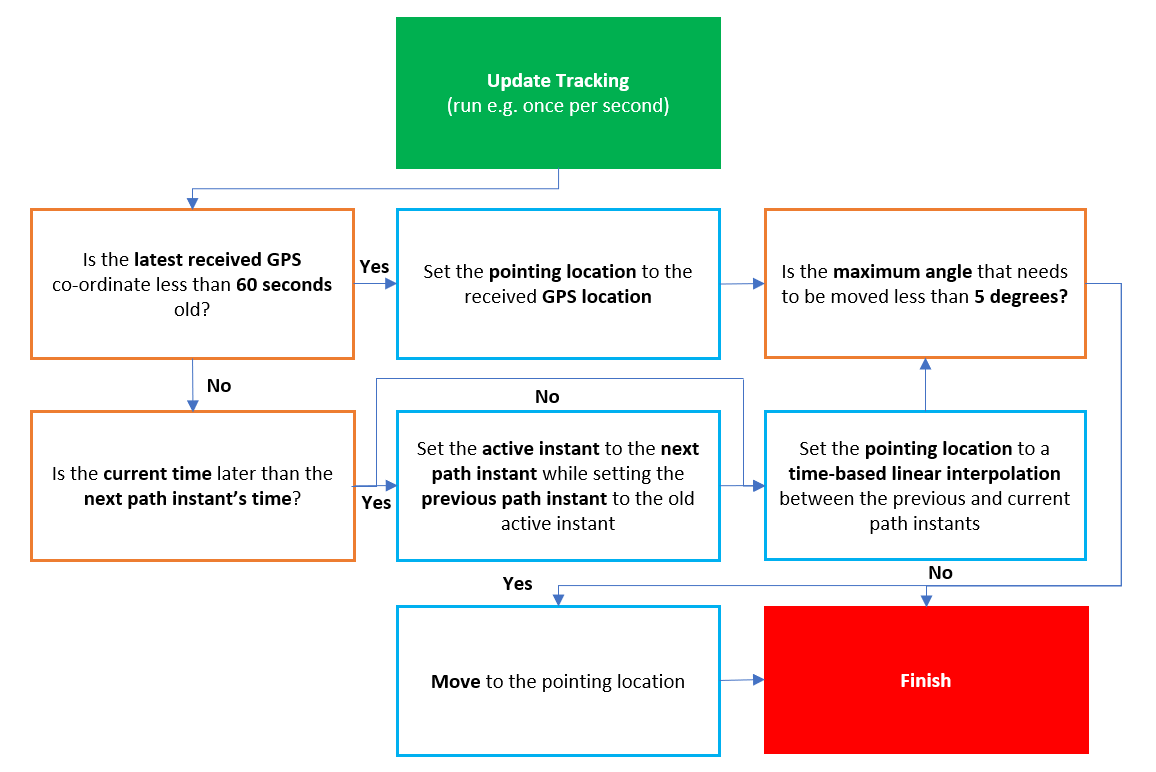
\includegraphics[width=0.98\textwidth]{trackingAlgorithm}
  \caption{Tracking Algorithm Flow Diagram}
  \label{fig:trackingAlgorithm}
\end{figure}